\subsection{3. Свойства класса автоматных языков. Замкнутость относительно булевых операций.}

\Def Полный ДКА.
Полный ДКА (ПДКА) - ДКА, для которого выполнено:
$$\forall a \in \Sigma, q \in Q \,\,\, |\Delta (q, a)| = 1$$

\Statement Для любого автоматного языка $L$ существует ПДКА $M$, такой что $L(M) = M$ (т.е. автоматы распознают одинаковое множество слов);

Метод построения ПДКА из ДКА:\\
1) строим ''стоковую'' вершину.\\
2) Добавляем из всех вершин переходы по недостающим буквам в "сток".

\begin{figure}[h]
    \hspace{-4ex} \begin{minipage}[h]{1\linewidth}
    \center{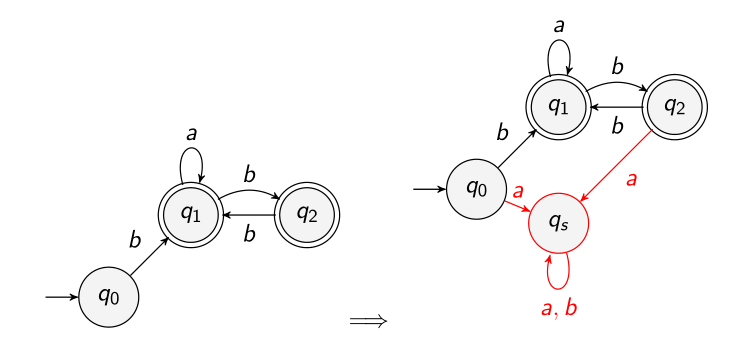
\includegraphics[width=0.6\linewidth]{1_3_1.png}}
    \end{minipage}
    \hspace{-4ex}
\end{figure}

Появятся ли новые слова? - нет, потому что, если мы попали в стоковую вершину, то не сможем ''выбраться'' из неё.

\Def Итерация Клини для языка L.
$$L^* = \cup_{k = 0}^{\infty}L^k$$

\Th Класс автоматных языков замкнут относительно\\
1. Конкатенации\\
2. Объединения\\
3. Пересечения\\
4. Итерации Клини\\
5. Дополнения

\Proof
Далее будем рассматривать только НКА с одним завершающим состоянием.
Для того чтобы после операции у итогового автомата было одно завершающее состояние, добавляем состояние и соединяем завершающие состояния с ним с помощью $\varepsilon$-переходов. (делаем новое состояние - завершающим, а старые - не завершающими)

1) Конкатенация $M_1$ и $M_2$:

Соединяем $\varepsilon$-переходами завершающее состояние $M_1$ со стартовыми состояниями $M_2$.
\begin{center}
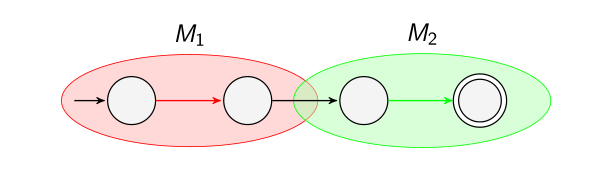
\includegraphics[width=0.45\linewidth]{1_3_2.png}
\end{center}

2) Объединение $M_1$ и $M_2$:

Добавляем стартовое состояние. Соединяем её со стартовыми состояниями $M_1$ и $M_2$ с помощью $\varepsilon$-переходов. 
\begin{center}
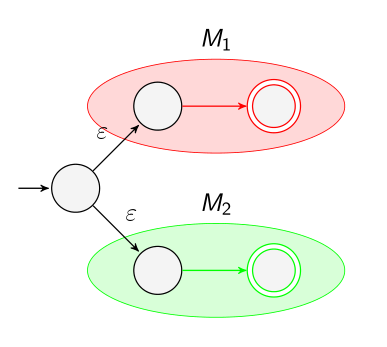
\includegraphics[width=0.25\linewidth]{1_3_3.png}
\end{center}

4) Итерации Клини над $M_1$:

Добавляем стартово-завершающее состояние. С помощью $\varepsilon$-переходов соединяем её с начальными состояниями $M_1$, а завершающее состояния $M_1$ с ней.
\begin{center}
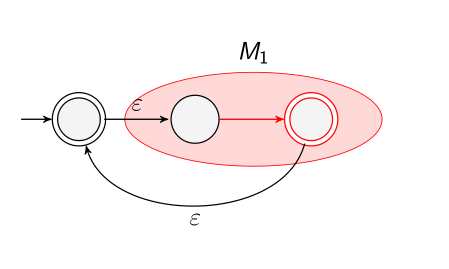
\includegraphics[width=0.32\linewidth]{1_3_4.png}
\end{center}

3) Пересечение $M_1$, $M_2$:

Строим "декартово произведение" автоматов с одно буквенными переходами.

\begin{center}
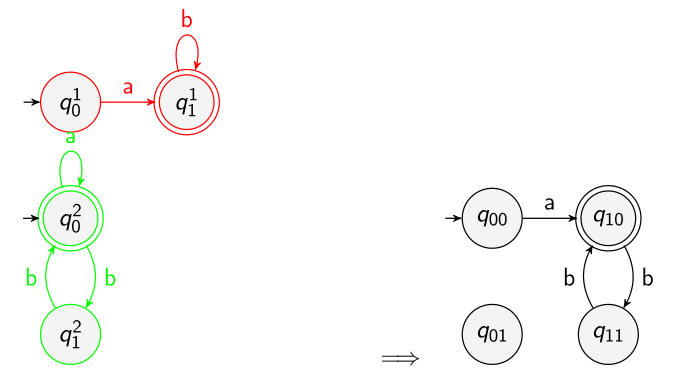
\includegraphics[width=0.55\linewidth]{1_3_5.png}
\end{center}

То есть пересечение будет состоять из состояний, каждому из которых соответствует пара чисел $(i, j)$, это номера состояний из $M_1$ и $M_2$ соответственно, которым это состояние соответствует. И между состояниями $(i_1, j_1)$ и $(i_2, j_2)$ будет проходить ребро с символом $k$, если между $i_1$ и $i_2$ проходило ребро с символом $k$ в $M_1$ и между $j_1$ и $j_2$ проходило ребро с символом $k$ в $M_2$. $(i, j)$ - стартовое состояние, если $i$ - стартовое в $M_1$, $j$ - стартовое в $M_2$. Аналогично с завершающем состоянием. 

5) Дополнение: строим ПДКА и инвертируем терминальность всех состояний.
